\typeout{IJCAI--PRICAI--20 Instructions for Authors}

% These are the instructions for authors for IJCAI-20.

\documentclass{article}
\pdfpagewidth=8.5in
\pdfpageheight=11in
% The file ijcai20.sty is NOT the same than previous years'
\usepackage{ijcai20}

% Use the postscript times font!
\usepackage{times}
\usepackage{soul}
\usepackage{url}
\usepackage[hidelinks]{hyperref}
\usepackage[utf8]{inputenc}
\usepackage[small]{caption}
% \usepackage{graphicx}
% \usepackage{amsmath}
% \usepackage{amsthm}
% \usepackage{booktabs}
% \usepackage{algorithm}
% \usepackage{algorithmic}
\urlstyle{same}

% The preceding line is only needed to identify funding in the first footnote. If that is unneeded, please comment it out.
\usepackage{cite}
%\usepackage{amsmath,amssymb,amsfonts}
%\usepackage{algorithmic}
\usepackage{graphicx}
\usepackage{textcomp}
\usepackage{xcolor}

\usepackage{enumerate}
\usepackage{caption}
\usepackage{subcaption}
\usepackage{graphicx}
\graphicspath{{figures/}}
%\graphicspath{{pdf/}}
\usepackage{mathtools,commath,amsmath,amssymb,amsfonts,bm}\interdisplaylinepenalty=2500
\usepackage{amsthm}
\usepackage{algpseudocode,algorithm}
\usepackage{tabularx,adjustbox}
\usepackage{todonotes}
\usepackage{breqn}
%\usepackage{color,cite}
\clearpage
\extrafloats{100}
\RequirePackage{tcolorbox}
\tcbuselibrary{breakable}
\tcbset{parbox=false, left=1ex, right=1ex}

\usepackage{multirow}
\usepackage{xspace}
\usepackage{url}
\newcolumntype{C}[1]{>{\hsize=#1\hsize\centering\arraybackslash}X}

\def\vec#1{\mathchoice{\mbox{\boldmath$\displaystyle#1$}}
  {\mbox{\boldmath$\textstyle#1$}}
  {\mbox{\boldmath$\scriptstyle#1$}}
  {\mbox{\boldmath$\scriptscriptstyle#1$}}}
\newcommand{\mat}[1]{\mathbf{#1}}
\newcommand{\isdefinedas}{\overset{\mathrm{def}}{=}}
\newcommand{\Set}[1]{\mathcal{#1}}
\newcommand{\definedas}{\overset{\mathrm{def}}{=}}
\newcommand{\etal}{\textit{et~al.}\xspace}
\newcommand{\ie}{\textit{i.e.},\xspace}
\newcommand{\eg}{\textit{e.g.},\xspace}
\newcommand{\mech}{\ensuremath{\mathcal{M}}\xspace}
\newcommand{\nbeg}[1]{\todo[noline,size=\tiny,backgroundcolor=yellow]{#1}\cbstart}
\newcommand{\nend}{\cbend}

\newtheorem{theorem}{Theorem}
\newtheorem{corollary}{Corollary}
\newtheorem{lemma}{Lemma}
\newtheorem{exmp}{Example}[section]
\newtheorem{definition}{Definition}

\DeclareMathOperator{\DDP}{DDP}
\algnewcommand\algorithmicinput{\textbf{Input:}}
\algnewcommand\Input{\item[\algorithmicinput]}
\algnewcommand\algorithmicoutput{\textbf{Output:}}
\algnewcommand\Output{\item[\algorithmicoutput]}
\algnewcommand\algorithmictier{\textbf{Role:}}
\algnewcommand\Tier{\item[\algorithmictier]}
\renewcommand{\algorithmicrequire}{\textbf{Input:}}
\renewcommand{\algorithmicensure}{\textbf{Parameters:}}

\title{Targeting Collaborative Fairness in Federated Learning}% to Business
%\title{Enhancing Efficiency and Fairness of Federated Learning with Sketching}

%\author{\IEEEauthorblockN{Lingjuan~Lyu}
%\IEEEauthorblockA{\textit{dept. name of organization (of Aff.)} \\
%\textit{name of organization (of Aff.)}\\
%City, Country \\
%email address or ORCID}
%\and
%\IEEEauthorblockN{2\textsuperscript{nd} Given Name Surname}
%\IEEEauthorblockA{\textit{dept. name of organization (of Aff.)} \\
%\textit{name of organization (of Aff.)}\\
%City, Country \\
%email address or ORCID}
%\and
%\IEEEauthorblockN{3\textsuperscript{rd} Given Name Surname}
%\IEEEauthorblockA{\textit{dept. name of organization (of Aff.)} \\
%\textit{name of organization (of Aff.)}\\
%City, Country \\
%email address or ORCID}
%\and
%\IEEEauthorblockN{4\textsuperscript{th} Given Name Surname}
%\IEEEauthorblockA{\textit{dept. name of organization (of Aff.)} \\
%\textit{name of organization (of Aff.)}\\
%City, Country \\
%email address or ORCID}
%\and
%\IEEEauthorblockN{5\textsuperscript{th} Given Name Surname}
%\IEEEauthorblockA{\textit{dept. name of organization (of Aff.)} \\
%\textit{name of organization (of Aff.)}\\
%City, Country \\
%email address or ORCID}
%\and
%\IEEEauthorblockN{6\textsuperscript{th} Given Name Surname}
%\IEEEauthorblockA{\textit{dept. name of organization (of Aff.)} \\
%\textit{name of organization (of Aff.)}\\
%City, Country \\
%email address or ORCID}
%}

\begin{document}
\maketitle

\begin{abstract}
In current deep learning paradigms, the standalone framework tends to result in overfitting and low utility. This problem can be addressed by %either a centralized framework that deploys a central server to train a global model on the joint data from all parties, or a distributed 
collaborative/federated learning that leverages a parameter server to aggregate local model updates. However, all the existing collaborative learning frameworks have overlooked an important aspect of participation: collaborative fairness. In particular, all parties can get same or similar models, even the ones who contribute nearly nothing. To address this issue, we make the first-ever investigation on the collaborative fairness, and propose a novel reputation-based method to facilitate fairness in collaborative learning. %We make the first-ever investigation on the collaborative fairness in collaborative learning, and exams a novel reputation-based strategy to guarantee fairness. 
We experimentally demonstrate that using our proposed method, fairness and accuracy in federated learning can be effectively achieved at the same time. Moreover, our framework provides a viable solution to detect and isolate the low-reputation party such as the free-riders in the collaborative learning system.
\end{abstract}

%\begin{IEEEkeywords}
%Collaborative Learning, Fairness, Reputation.
%\end{IEEEkeywords}

\section{Introduction}
Training complex deep networks on large-scale datasets is computationally expensive and may not be feasible for a single party in practice. Moreover, the data owned by a single party may be very homogeneous, resulting in overfitting which negatively impacts accuracy when the model is applied to previously unseen data, \ie poor generalizability. Therefore, there is a high demand to perform federated learning~\cite{FL2019}. 

In the current federated learning paradigm~\cite{mcmahan2016federated}, all participants receive the same federated model at the end of collaborative model training regardless of their contributions. This is obviously unfair, because all parties including the low-contribution parties can get the same global model. However, in reality, some parties may contribute more compared with other parties, while some parties may contribute nearly nothing or even negatively. This also makes the paradigm vulnerable to free-riding participants. For example, several banks may want to work together to build model to predict the creditworthiness of small and medium enterprises. However, but larger banks with more data maybe reluctant to train their local model based on high quality local data for fear of smaller banks benefiting from the shared FL model and eroding its market share~\cite{FL2019}. Without the guarantee of privacy and the promise of collaborative fairness, participants with high quality and large datasets may be discouraged from joining federated learning, thereby negatively affect the formation of a healthy FL ecosystem. Existing research on fairness mostly focuses on protecting sensitive attributes or reducing the variance of the prediction distribution across participants~\cite{cummings2019compatibility,jagielski2018differentially}. The problem of treating federated learning participants fairly remains open~\cite{FL2019}.

To overcome this problem, it is essential to develop a fair federated learning framework that respects collaborative fairness and accuracy at the same time. In this paper, we address the problem of treating FL participants fairly based on their contributions to build a healthy FL ecosystem. We refer to the proposed framework as the Collaborative Fair Federated Learning (CFFL) framework. Unlike existing work such as~\cite{Yu-et-al:2020AIES} which uses monetary rewards to incentivize good behaviour, our proposed solution fundamentally changes the current FL paradigm so that participants may not receive the same FL model in the end. Instead, each of them will receive a final FL model with performance reflecting their individual contributions to the federation. CFFL achieves collaborative fairness through the evaluation of reputation that considers the contribution of each party during collaborative learning process. 

To the best of our knowledge, this paper is the first to achieve collaborative fairness in federated learning through adjusting the level of performance of the version of the FL model allocated to each participant based on his contribution. Extensive experiments based on benchmark datasets %under two realistic scenarios in both homogeneous and heterogeneous settings 
demonstrate that CFFL achieves high fairness, delivers comparable accuracy to existing %centralized and 
distributed deep learning framework, and outperforms standalone deep learning framework.

%lack of fairness might discourage collaboration among parties. To the best of our knowledge, all the current research works of fairness focus on the protection of some specific attributes, or aim to reduce the variance of the accuracy distribution across participants~\cite{cummings2019compatibility,jagielski2018differentially}, while none of the previous works addressed the problem of collaborative fairness and privacy at the same time. To overcome these problems, it is essential to develop a fair and privacy-preserving collaborative learning framework that respects collaborative fairness, data privacy and utility at the same time. Moreover, we adopt an honest-but-curious setting: each party is assumed to be curious in inferring sensitive information of other parties; and yet, it is assumed to be honest in operations. This setting is reasonable as in our scenario parties are considered as organisations such as financial or biomedical institutions acting with responsibilities by laws. However, we also discuss how our design can help prevent certain behaviours of the insider attacker, and resist the outsider attacker in Section~\ref{sec:Discussion}. 

%~\cite{kuo2019fair} studied fairness problem of load sharing in blockchain-based privacy-preserving learning, ~\cite{li2019fair} formulated fairness as a more uniform accuracy distribution in federated learning, these works are all different from the collaborative fairness in our work. 


%In summary, all the existing collaborative frameworks (distributed or decentralized) focus on how to learn a global model or multiple local models with higher accuracy than individual standalone models, neglecting an important motivation for collaboration: \textbf{collaborative fairness}. 

%In particular, we want to remark that there is no concrete definition of collaborative fairness in both the standalone framework and the centralized framework, because parties do not collaborate in the standalone framework, and parties cannot get access to the trained global model in the centralized framework, %they can only get the prediction result in the name of 
%as the global model is only available in the form of ``machine learning as a service" (MLaaS). However, in distributed framework, all parties can fetch the same global model from the central server. This framework ais obviously unfair, because all parties including the low-contribution parties can get the same global model. However, in reality, some parties may contribute more compared with other parties, while some parties may contribute nearly nothing or even negatively. %high-quality data (\eg data with more diversity and high-quality annotations) 
%This is obviously unfair, because all parties including the low-contribution parties can get the same global model. However, in reality, some parties may contribute more compared with other parties, while some parties may contribute nearly nothing or even negatively. 
%The reason lies in the fact that different parties may have different capacities to generate the training data, and there may exist unpredictable random errors during data collection and storage. On the other hand, different parties have different sharing levels, some parties are more willing to share their information, while some are more private.
%However, all the current collaborative deep learning frameworks allow all parties including the low-contribution parties to get the same global model. 
%Hence, in independent and identically distributed (IID) setting, contribution can be quantified by either "data size" or "sharing level", and the high-contribution party has more data and higher sharing level.  

The rest of this paper is organized as follows. Section~\ref{sec:Related_work} reviews the related literature on fairness in federated learning which are major problems we aim to tackle. Section~\ref{sec:CFFL} presents technical details of the proposed CFFL framework. Section~\ref{sec:Performance} evaluates the performance of CFFL in terms of accuracy and fairness for different SGD frameworks% under different settings
, followed by discussions in Section~\ref{sec:Discussion}. Section~\ref{sec:Conclusion} concludes the paper and points out potential future research directions. 

%horizontal FML setup where we use deletion method for indicating group instance importance
%We first calculated the Shapley value for the whole feature space, as shown in Fig. 3, which directly reflects the importance for different features as normal Shapley value indicates.

%We then simulated the vertical FML for multiple participants, where we evenly separate the 15 features into 5 groups and each group represents a single participants with 3 features. Each time we group the features from one party together as the federated feature, and run the Shapley value algorithms to calculate the feature importance for this single federated feature together with the other individual features from the other participants. 
%use federated features all together for all the participants and calculate the Shapley value at one go. We expect that this will give less accurate results. Vertical FML setup, federated Shapley value is a good quantity to indicate the contribution for each participant.

%Horizontal FML and Vertical FML by using group instance deletion and group Shapley values.
%Our experiment results indicate that our method is effective and can give fair and reliable contribution measurements for FML participants without disclosing the data and breaking the initial intent of preserving data privacy.


%Our work for contribution measurement for FML participants is model agnostic, meaning that this should work for almost any kind of machine learning algorithms, and become a general framework for this task.

%influential functions [8] for horizontal FML and for some sampling version of calculating Shapley values for vertical FML. Those algorithms will help get an accurate and fair contribution measurement results with higher computational efficiency.

%the value of each training point needs to be updated and accumulated on the fly. Monte Carlo-based approximation algorithms. The central idea behind these approximation algorithms is to treat the Shapley value of a training point as its expected contribution to a random subset and use the sample average to approximate the expectation. 
%%%%%%%%%%%%%%%%%%%%%%%%%%%%%%%%%%%%%%%%
\section{Related Work}
\label{sec:Related_work}
In this section, we review relevant literature on fairness in federated learning to position our research in relation to existing research.
%\subsection{Fairness in Federated Learning}
Existing approach for promoting collaborative fairness among federated learning participants is based on incentive schemes. In general, participants shall receive payoffs that is commensurate with their contributions. Equal division is an example of egalitarian profit-sharing \cite{Yang-et-al:2017IEEE}. Under this scheme, the available total payoff at a given round is equally divided among all participants. Under the Individual profit-sharing scheme \cite{Yang-et-al:2017IEEE}, each participant $i$'s own contribution to the collective (assuming the collective only contains $i$) is used to determine his share of the total payoff.

The Labour Union game \cite{Gollapudi-et-al:2017} profit-sharing scheme determines a participant's share of the total payoff based on his marginal contribution to the utility of the collective formed by his predecessors (i.e. each participant's marginal contribution is computed based on the same sequence as they joined the federation). The Fair-value game scheme \cite{Gollapudi-et-al:2017} is a marginal loss-based scheme. Under this scheme, a participant's share of the total payoff is determined by the sequence following which the participants leave a federation. The Shapley game profit-sharing scheme \cite{Gollapudi-et-al:2017} is also a marginal contribution-based scheme. Unlike the Labour Union game, Shapley game aims to eliminate the effect of the participants joining the collective in different sequences in order to more fairly estimate their marginal contributions to the collective. Thus, it averages the marginal contribution for each participant under all different permutations of him joining the collective relative to other participants. This approach is computationally expensive.

For gradient-based federated learning approaches, the gradient information can be regarded as a useful source of data. However, in these cases, output agreement-based rewards are hard to apply as mutual information requires a multi-task setting which is usually not present in such cases. Thus, among these three categories of schemes, model improvement is the most relevant way of designing rewards for federated learning. There are two emerging federated learning incentive schemes focused on model improvement.

%A scheme which pays for marginal improvements brought about by model updates was proposed in \cite{Richardson-et-al:2019}. The sum of improvements might result in overestimation of contribution. Thus, the proposed approach also includes a model for correcting the overestimation issue. This scheme ensures that payment is proportional to model quality improvement, which means the budget for achieving a target model quality level is predictable. It also ensures that data owners who submit model updates early receive a higher reward. This motivates them to participate even in early stages of the federated model training process. %Similar to \cite{Richardson-et-al:2019}, \cite{Jia-et-al:2019} computes a Shapley value to split reward among data owners. %Such computations tend to be expensive. In addition, it does not address the issue that the same dataset can be contributed without extra cost to multiple federations.

In addition to the contributions made by participants, \cite{Yu-et-al:2020AIES} proposed a joint objective optimization-based approach to take costs and waiting time into account in order to achieve additional notions of fairness when distributing payoffs to FL participants. Different from the aforementioned approaches, the proposed CFFL framework does not utilize monetary payoffs to achieve fair treatment of FL participants. Instead, it allocates each of them a different version of the FL model with performance commensurate with his contributions. This represents a alternative paradigm to existing federated learning in which all participants receive the same final FL model.

%\section{The Proposed Method}
\section{The CFFL Framework}
\label{sec:CFFL}
\subsection{Collaborative Fairness Definition}
%The fundamental principle behind fairness is that the high-contribution party %party who invests more time and effort to collect high-quality data 
%should be rewarded more than the low-contribution party. A intuitive definition for collaborative fairness is given in Definition~\ref{def:fairness}.
The contribution difference lies in the fact that different parties may have different capacities to generate the training data, and there may exist unpredictable random errors during data collection and storage. On the other hand, different parties have different sharing levels, some parties are more willing to share their information, while some are more private. 
Since our focus here is to distribute different variants of the final FL model to participants based on their contributions, the notion of fairness most relevant for our purpose is \textit{Fairness through Awareness}. %Under this notion, individuals who are similar with respect to a similarity metric defined for a particular task should receive a similar outcome~\cite{Mehrabi-et-al:2019}. 
Unlike the traditional distributed/federated learning, where all parties can have access to the same global model, our design does not force a single global model onto local models. Instead, each local model is updated separately by improving their local accuracy. Therefore, parties finally converges to different local models, thus ensuring fairness. %enables fairness by enforcing each party to converge to different final models. %have access to a fraction of global model as per its reputation.
The fundamental principle behind fairness is that a party with high-contribution should be rewarded more than a party with low-contribution party. Under this context, we define collaborative fairness as:

\begin{definition}\label{def:fairness}
Collaborative fairness. In collaborative learning systems, a high-contribution party is deserved to be rewarded with a better performing local model than a low-contribution party. Specially, fairness can be quantified by the correlation coefficient between the contributions of parties and their respective final model accuracies. 
\end{definition}



%Policy to share: Different users may have different preferences over what kind of noise can be added to their public data. For instance, in recommender systems, a user may prefer modifying its existing rating scores, while another user may prefer adding new rating scores. We call a policy specifying what kind of noise can be added a noise-type-policy. In particular, we consider the following three types of noise-type-policy.



\subsection{Fairness via Reputation}% empowers fairness
%Correlation with RONI. A Reject on Negative Influence (RONI) defense~\cite{barreno2010security} counters ML poisoning attacks. When evaluating a set of suspicious training examples, this defense trains two models: one model using a trusted dataset, and another model using the union of the trusted and suspicious data. If the performance of the model degrades the performance beyond a specified threshold, the data is rejected.
%
%extend RONI to a federated learning setting, the server can capture the influence of a single update, rather than an entire dataset. RONI is ineffective in this setting because, at any given iteration, an honest gradient may update the model in an incorrect direction, resulting in a drop in validation accuracy.
%
%Depending on the RONI threshold, this poisoning attack may go undetected.
%We show that using RONI with a validation dataset that contains a uniform distribution of data, is insufficient in countering sybil-based poisoning in a non-IID setting. In the non-IID setting, clients send updates that do not represent an update from the global data distribution. Validating individual updates from a single client in such a manner produces false positives because the aggregator holds a validation set that contains uniform samples, and RONI flags each of their updates as malicious for doing poorly on the validation set.
%Without prior knowledge of the details of a potential attack, RONI is unable to distinguish between updates coming from sybils and updates coming from honest non-IID clients.
%
%shows the total sum of the RONI score across all iterations
%A RONI score below 0 indicates rejection. 
%
%existing defenses against malicious adversaries in ML (Multi-Krum [10] and RONI [6] (shown in Appendix B)) are inadequate.
%
%A RONI (Reject on Negative Influence) defense [3] counters ML poisoning attacks. Given a set of un- trusted training examples Dun, this defense trains two models, one model using all of the trusted training data D, and another model using the union dataset D? = D ? Dun which includes the untrusted data. If the performance of D? is significantly worse than the performance of D on a validation dataset, the data Dun is flagged as malicious and rejected. However, this defense relies on access to the centralized dataset, which is infeasible in the federated learning setting.
%
%We develop a distributed RONI defense that uses sets of gradient updates, instead of datasets, and independently evaluates the influence that each gradient update has on the performance of a trusted global model. Validation (Algorithm 2) executes within the parameter server and validates that iterations performed by clients have a positive impact. Validation is parameterized by two variables: the validation rate at which validations are performed, and the RONI threshold [3] required before a client is flagged.
%
%Dancing in the Dark: Private Multi-Party Machine Learning in an Untrusted Setting:
%To ensure that validations are performed in a fair manner, we benchmark all clients against the same candidate model. The validator intersperses validation iterations within the gradient updates requests in distributed SGD. A validation round is triggered through a periodic Bernoulli test, with the probability parameterized by a validation rate. During a validation round, the current model state is snapshotted, and
%a copy of this model is sent to all active clients. The clients' gradient responses are collected and the RONI value is calculated and accumulated.
%
%When the rate of validation is increased, the server discovers poisoning clients more quickly, but with a performance overhead. When the RONI threshold is increased, the server is more likely to detect adversaries, but the false positive rate of flagging honest nodes increases as well.
%An important design detail is that a validation request looks just like a gradient update request.
%
%Validation is parameterized by two variables: the validation rate at which validations are performed, and the RONI threshold [3] required before a client is flagged.
%RONI threshold is maintained at 2\%.
%validation rate of 0.1
%RONI threshold is varied from 0.5\% to 5\%.
%
%Figure 11 shows the execution of model training with 50\% poisoning clients for different RONI validation thresholds. As the threshold decreases, adversaries are removed from the system more quickly, allowing the model to recover from the poisoning damage.
%Setting the RONI threshold too low is also dangerous as it increases the effect of false positives. In Figure 11, we observe that the model initially performs poorly, this is due to incorrectly penalizing honest clients. 
%
%
%\emph{A Reject on Negative Influence} (RONI)~\cite{barreno2010security} with a validation dataset that contains a uniform distribution of data
%at any given iteration, an honest gradient may update the model in an incorrect direction, resulting in a drop in validation accuracy. This is confounded by the problem that clients may have data that is not accurately modeled by the RONI validation set

%We audit the contribution of each party based on a characterization of the influence that party updates have on the validation accuracy in each communication round. 

During collaborative learning process, the server audits the claims of each party based on a characterization of the influence of its local model updates %have 
on the validation accuracy in each communication round. 
%verifies the claims of other parties and 
The server keeps a reputation list, and updates the reputations of all parties as per the contributions of their released gradients. In this way, the reputation of each party keeps changing, reflecting real-time contribution and thus delivering better fairness. The high-contribution party will be highly rated by the server, while the low-contribution party will be detected or even isolated from the collaborative learning system, avoiding the low-contribution party from dominating the whole system.

%In particular, we clarify that the low-contribution parties are not malicious, \ie they follow the protocol honestly and aim to benefit from other parties' data, but contribute lowly, or even nearly nothing or negatively.


%Our method ensures fairness during download and upload processes as follows:
%\begin{itemize}
%\item  \textbf{Download as per reputation}: 
%Since one party might contribute differently to different parties, the reputation of this party might be different from the view of different parties, therefore, each party $i$ should keep a local reputation list by sorting all parties as per their local reputations in the descending order, known only by party $i$ itself. The higher the reputation of party $j$ in party $i$'s reputation list, the more likely party $i$ will download gradients from party $j$, and consequently, more points will be rewarded to party $j$.
%
%\item  \textbf{Upload as per request and sharing level}: Once the server receives download request for gradients, how many meaningful gradients will be released is dependent on the reputation of the requester.
%\end{itemize}


In our CFFL framework, %to audit party updates, 
the server uses leave-one-out strategy to quantify the reputation of party $j$ based on the usefulness of party $j$'s gradients in each communication round. Specifically, the server evaluates the change of validation accuracy by removing party $j$'s gradients from the updated model parameter $\vec{w}_t'$ that combines all parties' gradients, \ie using the combined gradients with and without party $j$'s gradients to evaluate the validation accuracy, which yield $acc$ and $acc_j$ respectively, the difference between $acc$ and $acc_j$ reflects how party $j$ affects validation accuracy. The server computes the reputation $c_j$ of party $j$ at the current communication round by passing an "accuracy factor" $x=\frac{acc}{acc+acc_j}$ through a sigmoid function $f$ in Eq.~\eqref{eq:reputation}.
\begin{equation}\label{eq:reputation}
	c_j=f(x)=\frac{1}{1+exp(-15*(x-0.5))}
\end{equation}
% where $x=\frac{acc}{acc+acc_j}$ is termed as "accuracy factor". 
%The incentive can be explicitly explained as follows. As 
Here $x$ stands for the accuracy ratio between the validation accuracy using the combined gradients of all parties and the validation accuracy using the combined gradients excluding party $j$'s gradients, hence it can be further expressed as:
 \begin{equation}\label{eq:factor}
x=\frac{acc}{acc+acc_j}=\frac{acc}{2*acc+\Delta}
\end{equation}
where $acc_j=acc+\Delta$, $\Delta$ indicates the impact of removing party $j$, the more positive the value of $\Delta$, the better the validation accuracy after removing party $j$, hence the lower the contribution of party $j$. To be more specific, if party $j$ has no impact, $\Delta=0, x=0.5, c_j=0.5$; if party $j$ contributes negatively, $acc_j>acc$, then $\Delta>0, x<0.5, c_j<0.5$; if party $j$ contributes positively, $acc_j<acc$, then $\Delta<0, x>0.5, c_j>0.5$. The server computes reputation of each party based on the its contribution in each round, then integrates its historical reputation to update its reputation in the reputation list. %by %averaging over the reputation of current epoch and previous epoch. 
In the follow-up rounds, the number of the updated global parameter to be downloaded will be dependent on the reputation of each party. The higher the reputation of party $j$ in the reputation list, the more likely party $j$ will be allocated with a more complete model from the server.%sharing level, reputation and download budget.


\begin{algorithm}[ht]
\caption{Fairness-aware federated learning}\label{Algorithm:Fair_FL}
\small
\begin{algorithmic} 
%\State \textbf{Input: $C$, $\vec{w^g}$, $\Delta \vec{w}_j$, $\lambda_j$, $\vec{w}_i$, $V$}
%\State \textbf{Output: updated parameters $\vec{w}_i'$, reputation ${c_i}'$}
\Require $C$, $\vec{w_g}$, $\Delta \vec{w}_j$, $\lambda_j$, $\vec{w}_i$, $V$.
%\State At current epoch, suppose party $i$ aims to download total $d_i$ gradients from all parties in $C$, while party $j \in C \setminus i$ can at most upload $\lambda_j \times |\Delta \vec{w}_j|$ gradients. Server updates the reputation list based on the gradients of party $j \in C$ as follows:
\State In each communication round, each party sends gradients to the server, and server updates its reputation and determines how much this party can download. Each party is initialized with the same parameter to start with.

 \Tier Party $j$
 \If{$j \in C \setminus i$}
 \State Downloads the allocated global parameter $\vec{w_g^j}$ from server and replaces the corresponding elements in local model $\vec{w}_j$ with $\vec{w_g^j}$;
 \State  Runs SGD on local data and updates the local parameters as $\vec{w}_j'$;
 \State  Computes gradient vector $\Delta \vec{w}_j=\vec{w}_j'-\vec{w}_j$;
%  Conducts local training to compute gradients: 
%\State $d_j^i=min(c_i^j*d_i, \lambda_j*|\Delta \vec{w}_j|)$
\State $\lambda_j*\Delta \vec{w}_j$ are grouped into set $S$ as $\Delta (\vec{w}_j)^S$, which are selected according to the ``largest values" criterion:
%\textbf{largest values}: gradients of $\Delta \vec{w}_j$ 
sort gradients in $\Delta \vec{w}_j$, and upload $\lambda_j*\Delta \vec{w}_j$ of them, starting from the largest.
\EndIf

\Tier Server
%\State Initializes global parameters $\vec{w_g}$;
\State \textbf{Parameter update}:  $\vec{w}_g'=\vec{w}_g+{\textstyle\sum}_{j \in C} \Delta (\vec{w}_j)^S$. 
\For{$j \in C$}
\State ${\vec{w}_g^j}'=\vec{w}_g'-\Delta (\vec{w}_j)^S$, where $\vec{w}_g$ is the server's global parameters of previous epoch.
\State $acc \leftarrow (\vec{w}_g', V_i)$, $acc_j \leftarrow ({\vec{w}_g^j}', V_i)$
\State $x=\frac{acc}{acc+acc_j}$
\State ${c_j}'=\frac{c_j+f(x)}{2}$, where $f$ refers to the sigmoid reputation mapping function in Eq.~\eqref{eq:reputation}.
\EndFor
\State \textbf{reputation normalisation}: 
  ${c_j}'=\frac{{c_j}'}{{\textstyle\sum}_{j \in C} {c_j}'}$
\If{${c_j}'<c_{th}$}
	\State server flags party $j$ as "low-contribution" and removes it, then runs reputation normalisation again.
\EndIf
%\State \textbf{reputation normalisation}: If majority party report party $j$ as "non-credible", Blockchain removes party $j$ from credible party set $C$ and all parties remove party $j$'s model updates $\Delta (\vec{w}_j^i)^S$ from their updated $\vec{w}_i'$ and rerun reputation normalisation again.
%\vspace{2mm}
\end{algorithmic}
\end{algorithm}

\subsection{Quantification of Fairness}
In FL system, collaborative fairness should be quantified from the point of view of the whole system. In this work, we quantify collaborative fairness through the correlation coefficient between party contributions (\ie standalone model accuracy which characterizes the learning capability of each party on its own local dataset) %, and sharing level, which characterizes the sharing willingness of each party) 
and party rewards (\ie final model accuracies of different parties). 

Specifically, we take party contributions as the X-axis, which represents the contributions of different parties from the system view. In particular, %in Setting 2, 
we characterize different parties' contributions by their %sharing levels and 
standalone model accuracies, as the party who %is less private and 
has local data with better generalization empirically contributes more. %In Setting 1 and Setting 3, we characterize different parties' contributions by their standalone model accuracies, as the party who has local data with better generalization empirically contributes more. Moreover, in Setting 3, the party with more local data typically yields higher standalone model accuracy in IID scenarios. 
In summary, the X-axis can be expressed by Equation~\ref{eq:x_axis}, where $sacc_j$ denotes the standalone model accuracy of party $j$:%$\lambda_j$ and $sacc_j$ denote the sharing level and standalone model accuracy of party $j$ respectively: 
\begin{equation}\label{eq:x_axis}
\vec{x}=\{sacc_1,\cdots,sacc_n\}
%\resizebox{0.93\hsize}{!}{
%\vec{x}=
%\left\{\begin{array}{cl}
%\{\frac{\lambda_1}{\textstyle\sum \lambda_j},\cdots,\frac{\lambda_n}{\textstyle\sum \lambda_j}\}+\{\frac{sacc_1}{\textstyle\sum sacc_j},\cdots,\frac{sacc_n}{\textstyle\sum sacc_j}\},  & \mbox{Setting 2} \\
%\{sacc_1,\cdots,sacc_n\}, & \mbox{Setting 1\&3} 
%\end{array}\right.}
\end{equation}

Similarly, we take party rewards (\ie final model accuracies of different parties) as the Y-axis, as expressed by Equation~\ref{eq:y_axis}, $acc_j$ denotes the final model accuracy of party $j$:
\begin{equation}\label{eq:y_axis}
\vec{y}=\{acc_1,\cdots,acc_n\}
\end{equation}

As the Y-axis measures local model performance of different parties after collaboration, it is expected to be positively correlated with the X-axis to deliver good fairness. Hence, we formally quantify collaborative fairness in Equation~\ref{eq:fairness}:
\begin{equation}\label{eq:fairness}
r_{xy}=\frac{{\textstyle\sum}_{i=1}^n (x_i-\bar{x})(y_i-\bar{y})}{(n-1)s_xs_y}
\end{equation}
where $\bar{x}$ and $\bar{y}$ are the sample means of $\vec{x}$ and $\vec{y}$, $s_x$ and $s_y$ are the corrected standard deviations. The range of fairness is within [-1,1], with higher values implying good fairness. Conversely, negative coefficient implies poor fairness. 


\section{Experimental Evaluation}
\label{sec:Performance}
\subsection{Datasets}
% ~\cite{lecun1998gradient} ~\cite{netzer2011reading}
We implement experiments on two benchmark image datasets. The first is the MNIST dataset\footnote{\url{http://yann.lecun.com/exdb/mnist/}} for handwritten digit recognition consisting of 60,000 training examples and 10,000 test examples. Each example is a 32x32 gray-level image~\cite{shokri2015privacy}, with digits locating at the center of the image. The second is the Adult Census dataset, which includes 48,843 records with 14 sensitive attributes, including age, race, education level, marital status, and occupation, etc\footnote{\url{http://archive.ics.uci.edu/ml/datasets/Adult}}. This dataset is commonly used to predict whether an individual makes over 50K dollars in a year (binary). There are total total 48,842 records, with 24\% (11687) records over 50K, while the remaining 76\% (37155) under 50K. %We split total 48,842 records into 39,074 training examples and 9,768 test examples. 
We manually balance the dataset to have 11687 records over 50K and 11687 records under 50K, resulting in total 23374 records. Among which, we choose 80\% records as training set, while the remaining 20\% as test set. 
For all datasets, we randomly choose 10\% training examples as validation set. 

\subsection{Baselines}
We demonstrate the effectiveness of our proposed CFFL framework by comparison with the following two representative frameworks. %We omit the centralized framework as distributed framework achieves similar even better accuracy than the centralized framework~\cite{shokri2015privacy}. 
In all frameworks, stochastic gradient descent (SGD) is applied to each party.

\begin{enumerate}
    \item \textit{Standalone} framework assumes parties train standalone models on local dataset without any collaboration. This framework delivers maximum privacy, but minimum utility, because each party is susceptible to falling into local optima when training alone. In particular, we remark that there is no concrete definition of collaborative fairness in the standalone framework, because parties do not collaborate in this framework.
%    \item \textit{Centralized} framework: which allows a trusted server to have access to all participants' data in the clear, and train a global model on the combined data using standard SGD. Hence, it is a privacy-violating framework.
    \item \textit{Distributed} framework enables parties to train independently and concurrently, and chooses a fraction of parameters to be uploaded at each iteration. In particular, as demonstrated in~\cite{shokri2015privacy}, Distributed Selective SGD (DSSGD) can achieve even higher accuracy than the centralized SGD because updating only a small fraction of parameters at each round acts as a regularization technique to avoid overfitting by preventing the neural network weights from jointly ``remembering'' the training data. Hence, we take DSSGD for the analysis of the distributed framework and omit the centralized framework. %As DSSGD with round robin parameter exchange protocol results in the highest accuracy~\cite{shokri2015privacy}, we follow the round robin protocol for DSSGD, where participants run SSGD sequentially, each downloads a fraction of the most updated parameters from the server, runs local training, and uploads selected gradients; the next party follows in the fixed order. 
In particular, we follow~\cite{shokri2015privacy} to choose the upload rate $\theta_u=10\%$, then gradients are uploaded according to the ``largest values'' criterion. %Without loss of generality, we use DSSGD protocol for distributed framework. %DSSGD allows all parties to have access to the global model on the server, %Moreover, in round robin protocol, the last party who downloads parameters always gains much more information than the previous parties, 
%which is obviously unfair.
\end{enumerate}

\subsection{Experimental Setup}
%Test accuracy of the train model on various domains, as a function of training epochs for the

%We randomly initialize the local training dataset of each participant with 1\% of the entire dataset, i.e., 600 data samples for the MNIST.


%from various domains,
%on the validation set and report accuracy distributions on the testing set. 
%For all datasets, we randomly sample 10 devices each round. We tune the learning rate and batch size on FedAvg and use the same learning rate and batch size for all q-FedAvg experiments of that dataset.

For MNIST dataset, we take \emph{multi-layer perceptron} (MLP) as local model architecture. %, we consider two popular neural network architectures: \emph{multi-layer perceptron} (MLP) and \emph{convolutional neural network} (CNN), \textbf{these two model architectures are the same as in~\cite{shokri2015privacy}}. %The CNN model for MNIST stacks two convolutional layers with max-pooling and one fully connected layer with ReLUs. 
For local model training, we set the learning rate as 0.001, learning rate decay as 1e-7, and batch size as 1. In addition, to reduce the impact of different initializations and avoid non-convergence, each party is initialized with the same parameter $w_0$, then local training is run on individual training data to update local model parameter $\vec{w_i}$. The sharing level of each party is fixed to $0.1$.  To %speed up convergence
boost fairness, we let each party individually train 10 epochs before collaborative learning starts. For all the experiments, we empirically set the reputation threshold as %$c_{th}=\frac{1}{n}*\frac{2}{3}$ via grid search, where $n$ is the number of parties\nend. 
$c_{th}=\frac{1}{|C|-1}*\frac{2}{3}$ via grid search, where $|C|$ is the number of alive parties %, \ie credible parties 
in the system. %Next, we investigate two realistic settings as follows: 

%\textbf{Setting 1: Different sharing level, same data size:} in the second case, sharing level of each party is randomly sampled from $[0.1,1]$, and parties release meaningful gradients as per individual sharing level during collaboration. For each participant, we randomly sample $1\%$ of the entire database as local training data as above. When the data size is the same, less private party with higher sharing level would like to release more information, and thus be rewarded more;
%%\ie $600$ examples for MNIST and $1000$ examples for Adult;

%\textbf{Setting 2: Different data size, same sharing level:} in the third case, 
In FL, the data across different parties can be inherently heterogeneous, violating iid assumption. In particular, we consider two practical scenarios, data size imbalanced and class number imbalanced.
For data size imbalanced scenario, to simulate %the real case where different parties have 
different parties owing different amount of data, we follow a power law to randomly partition total \{3000, 6000, 12,000\} examples among \{5,10,20\} parties respectively. Similarly, for Adult dataset, total \{5000, 10000, 20000\} examples are randomly partitioned among \{5,10,20\} parties. 
%The %sharing level 
%upload rate of each party is fixed to $0.1$. %When the sharing level is the same, the party with more data would contribute more and be rewarded more.
We remark that the purpose of allocating $600$ MNIST examples for each party is to fairly compare with Shokri \etal~\cite{shokri2015privacy}, in which each party is allocated with 600 MNIST examples (small number of local examples to simulate data scarity which necessitates collaboration). Therefore, for MNIST, we simulate the total examples of 3000 (5 parties) up to 12,000 (20 parties). For larger datasets like 300,000 examples, it would require 500 parties, imposing heavy requirement on deployment, while delivering similar results.%analysis as in Sec.~\ref{sec:results}. 

For class number imbalanced scenario, 

\subsection{Experimental Results}
\label{sec:results}
%For collaborative fairness , we analyze the distributed framework with and without our reputation-based method. 
Table~\ref{tbl:MNIST_Adult_fairness} lists the calculated fairness of the distributed framework and our CFFL over MNIST and Adult datasets under different settings of \{5,10,20\} parties.%, with different architectures, different party numbers and different settings, as detailed in Section~\ref{sec:Setup}. 
All the fairness results %in different settings 
are averaged over five trails. As is evidenced by the high positive values of fairness, with all of them above 0.5, CFFL achieves reasonably good fairness, confirming the intuition behind fairness: the party who %is less private and has more training data delivers higher accuracy. 
contributed more is reward with a better model. In contrast, the distributed framework exhibits bad fairness with significantly lower values than that of CFFL in all cases, and even negative values in some cases, manifesting the lack of fairness in the distributed framework. This is because in the distributed framework, all the participating parties can get access to the same global model, no matter how much one party contributes, which is obviously unfair.

\begin{table}[ht]
\caption{Fairness of distributed framework and our CFFL over MNIST and Adult datasets under different party settings (P-$k$ indicates there are $k$ parties in the experiments).}%, with different model architectures, different party numbers (P-$k$) and different settings as described in Section~\ref{sec:Setup}.}
\label{tbl:MNIST_Adult_fairness}
\centering
\begin{tabularx}{\linewidth}{|c|X|X|X|X|}
\hline
\multirow{2}{*}{} & \multicolumn{2}{c|}{MNIST} & \multicolumn{2}{c|}{Adult}
\tabularnewline
\cline{2-5}
 & Distributed & CFFL & Distributed & CFFL
\tabularnewline
\hline
% & CNN & MLP & CNN & MLP & CNN & MLP & CNN & MLP
%\tabularnewline
%\hline
\textit{P5}  &-0.68 & \textbf{0.84} & &\textbf{}
\tabularnewline
\hline
\textit{P10} &-0.20 &\textbf{0.79}  & &\textbf{}
\tabularnewline
\hline
\textit{P20} &-0.27 &\textbf{0.84} & & \textbf{}
\tabularnewline
\hline
\end{tabularx}
\end{table}



\begin{table}[ht]
\caption{%Maximum 
Accuracy [\%] over MNIST and Adult of varying party number settings, achieved by %\emph{Centralized}, 
\emph{Standalone}, \emph{Distributed} (DSSGD) and our CFFL. %(three settings as described in Section~\ref{sec:Setup}) frameworks using MLP and CNN architectures. 
}
\label{tbl:MNIST_Adult_acc}
\centering
\begin{tabularx}{\linewidth}{|l|*{6}{C{1}|}}
\hline
\multirow{2}{*}{Framework} & \multicolumn{3}{c|}{MNIST} & \multicolumn{3}{c|}{Adult}
\tabularnewline
\cline{2-7}
 & P5 & P10 & P20 & P5 & P10 & P20 
\tabularnewline
\hline
%\textit{Centralized} 
%& 91.68 & 95.17 & 96.28 & 96.85 
%& 96.58 & 98.19 & 98.52 & 98.58
%\tabularnewline
%\hline
% \textit{DSSGD (round robin w/o DP)}
\textit{Distributed} 
& 92.03  &94.33  & 95.52
&  &   & 
\tabularnewline
\hline
\textit{Standalone} 
& 88.16 &89.41 &89.52 
&  &   & 
\tabularnewline
\hline
%\textit{CFFL (Setting 1)} 
\textit{CFFL} 
&92.82 & 94.06 &94.88
&  &   & 
\tabularnewline
\hline
%\textit{CFFL (Setting 2)}
%&91.92   &95.70   &95.94  &96.23
%&95.50   &97.34   &97.84  &98.14
%\tabularnewline
%\hline
\end{tabularx}
\end{table}

%As is evident from Figure 

Table~\ref{tbl:MNIST_Adult_acc} provides the accuracy on MNIST and Adult datasets of \{5,10,20\} parties using %three 
baseline frameworks in Section~\ref{sec:Setup}, and our proposed CFFL. %in three realistic settings in Section~\ref{sec:Setup}. 
Here we report the %average accuracy under the setting of same  sharing level, and use maximum 
best accuracy because our CFFL enables parties to converge to different local models after collaborative learning, and we expect the most contributive party derives a local model with maximum accuracy approximating the distributed framework. %Similarly, Table~\ref{tbl:Adult_CNN} provides the accuracy on Adult dataset. 
For both MNIST and Adult datasets, we show the worst accuracy for standalone SGD (minimum utility, maximum privacy). In particular, CFFL obtains comparable accuracy to the distributed framework using DSSGD, and always achieves higher accuracy than the standalone SGD. For example, as shown in Table~\ref{tbl:MNIST_Adult_acc}, for MNIST dataset of 20 parties, our CFFL achieves -95\% test accuracy, which is higher than the standalone SGD 89\%, and comparable to the distributed framework using DSSGD. 
  
The above fairness results in Table~\ref{tbl:MNIST_Adult_fairness}, and accuracy results in Table~\ref{tbl:MNIST_Adult_acc} demonstrate that \emph{our proposed CFFL achieves both reasonable fairness and comparable accuracy}. 

\textbf{Party Convergence}. To investigate the impact of our CFFL on individual convergence, Fig.~\ref{fig:mnist_p5p10_mlp_convergence} %and Fig.~\ref{fig:mnist_p10_mlp_convergence} 
further depicts the accuracy trajectory of each party when running Standalone framework and our CFFL %with MLP architecture track individual accuracy
over MNIST across 100 communication rounds. For the sake of brevity, we only report experimental results obtained for the collaboration among 5 parties and 10 parties. %in Setting 2 and Setting 3.
It can be observed that our CFFL consistently delivers better accuracy than the standalone model obtained by any individual party, at the cost of slower convergence and more fluctuation. However, most parties can converge within the first 20 rounds, except those with lower standalone accuracy. For example, in Figure~\ref{fig:mnist_p5p10_mlp_convergence} (d), party 1 and party 2 encounter higher fluctuations compared with the other parties with higher standalone accuracies. More importantly, these figures confirm that our CFFL enforces all parties to converge to different local models, which are better than their standalone models without any collaboration, thereby offering fairness as claimed. 


\begin{figure*}[!htp]
\centering
        \begin{subfigure}[ht]{0.23\textwidth}
                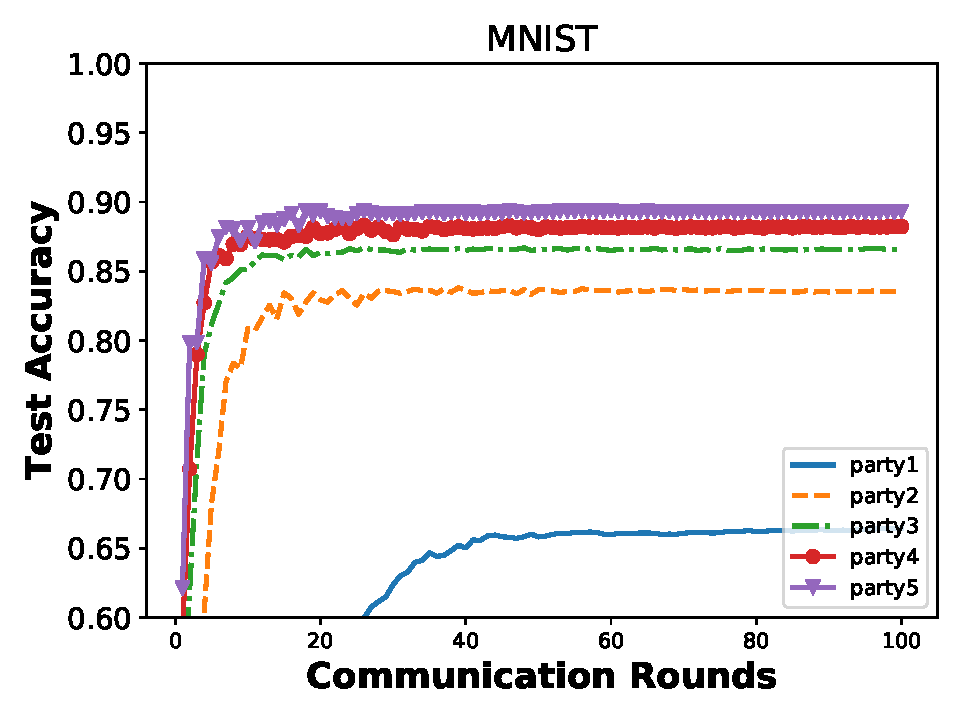
\includegraphics[width=4cm,height=3.8cm]{mnist_deep_p5e100_standalone}\label{fig:mnist_deep_p5e100_standalone}
                \subcaption{Standalone (P5)}
        \end{subfigure}
        \begin{subfigure}[ht]{0.23\textwidth}
                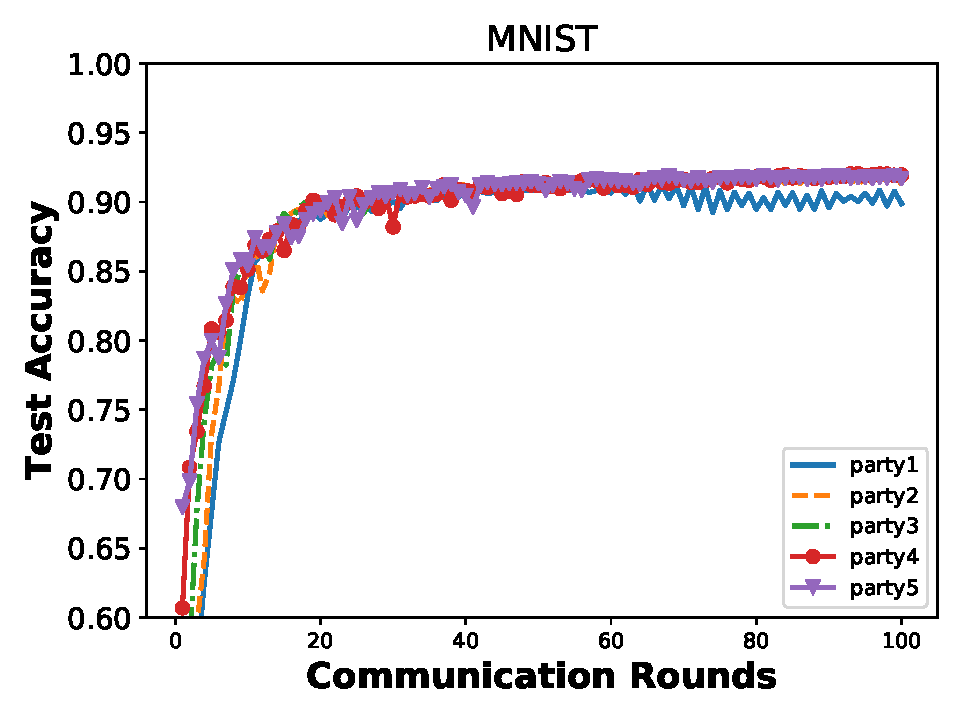
\includegraphics[width=4cm,height=3.8cm]{mnist_deep_p5e100_cffl}\label{fig:mnist_deep_p5e100_cffl}
                \subcaption{CFFL (P5)}
        \end{subfigure}
        \begin{subfigure}[ht]{0.23\textwidth}
                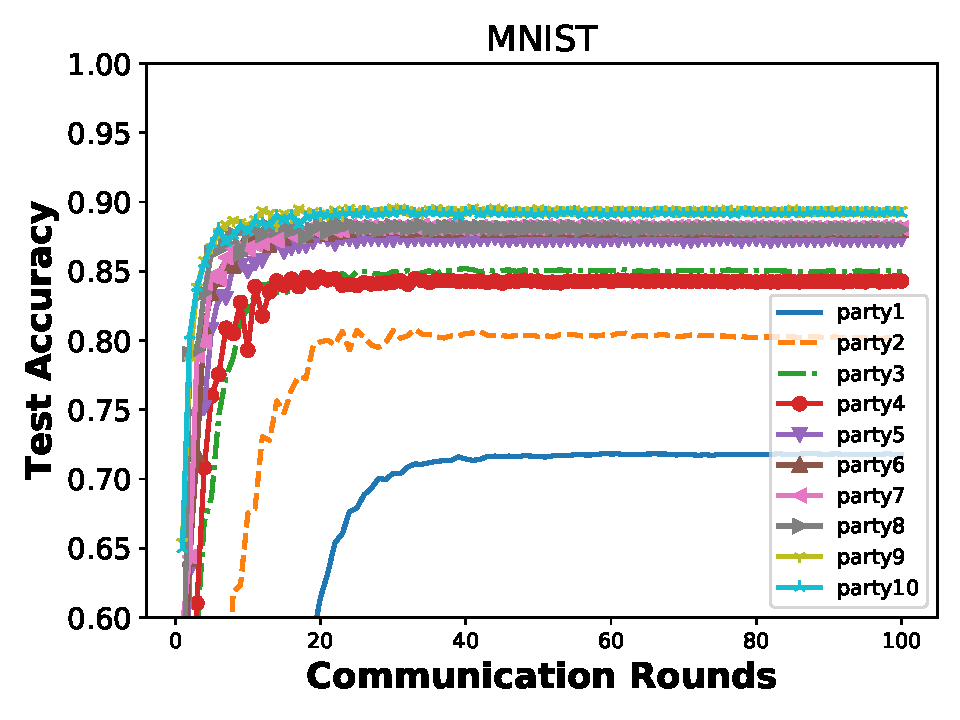
\includegraphics[width=4cm,height=3.8cm]{mnist_deep_p10e100_standalone}\label{fig:mnist_deep_p10e100_standalone}
                \subcaption{Standalone (P10)}
        \end{subfigure}
        \begin{subfigure}[ht]{0.23\textwidth}
                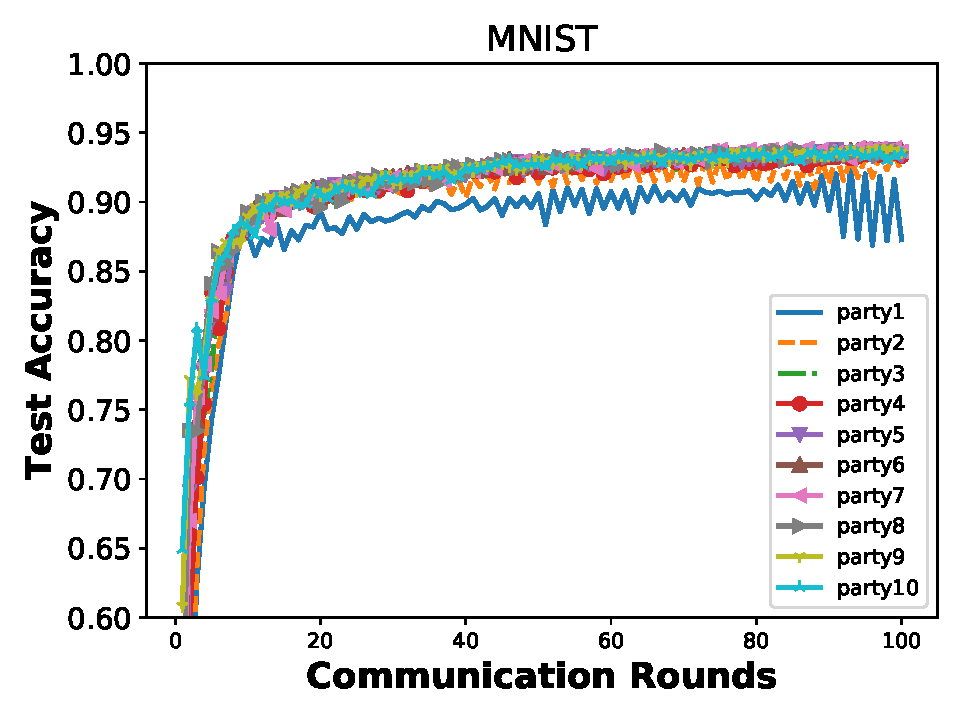
\includegraphics[width=4cm,height=3.8cm]{mnist_deep_p10e100_cffl}\label{fig:mnist_deep_p10e100_cffl}
                \subcaption{CFFL (P10)}
        \end{subfigure}
        \caption{Individual convergence for MNIST MLP using Standalone framework and our CFFL (B=1, E=1, lr=0.001).}%(Total 4 parties)
\label{fig:mnist_p5p10_mlp_convergence}
\end{figure*}

To speed up convergence and alleviate fluctuations, we further experiment with larger number of local epochs, larger local batch size, and higher learning rate. As corroborated by Fig.~\ref{fig:mnist_p4p15_cvn_convergence_localepoch5_localbatch10_lr0.15}, by setting $B=10, E=5, lr=0.15$, each party can converge faster, without affecting both accuracy and fairness. For example, for P10 in Figure~\ref{fig:mnist_p15_cvn_convergence} (d), it needs 65 communication rounds for all parties to converge using $B=1, E=1, lr=0.001$, while it only needs 50 communication rounds using $B=10, E=5, lr=0.15$ in Figure~\ref{fig:mnist_p4p15_cvn_convergence_localepoch5_localbatch10_lr0.15} (d). However, this faster convergence and less fluctuations come at the cost of local computation at each party.


%%%%%%%%%%%%%%%%%%%%%%%%%%%%%%%%%%%%%%%%
\section{Discussions}
\label{sec:Discussion}
\textbf{Fairness in heterogeneous settings.} 
Sharing model updates is typically limited only to homogeneous FL architectures, \ie the same model architecture is shared with all parties. In heterogeneous settings, parties may train different types of local model, instead of sharing model updates, parties can share model predictions on the unlabeled public dataset. The server then quantifies the reputation of each party based on their local prediction. We remark that sharing model predictions is model agnostic, meaning that this should work for almost any kind of machine architecture.
%is model agnostic, meaning that this should work for almost any kind of machine learning algorithms, and become a general framework for this task. 
We evaluate FL with heterogeneous model architectures, and show its effectiveness without compromising the final accuracy of party models.
We use Purchase data and 5 fully connected models, which we call M1, M2, M3, M4, and M5, with hidden layer sizes \{\}, \{1024\}, \{512, 256\}, \{1024, 256\}, and \{1024, 512, 256\} respectively. Note that, M1 has lower capacity, thus should deliver lower accuracy than the other four models.

%collaboration between models with heterogeneous architectures.
%After a few rounds of local training on their private data, the Cronus parties share their predictions on the public data.

\textbf{Reputation threshold}. If the server finds out that the reputation of one party is lower than the threshold $c_{th}$, implying a potentially low-contribution party, it will be isolated from the collaborative learning system. 
Here, $c_{th}$ is mainly used to detect and isolate the extremely low-contribution party, and it should be agreed by the majority of parties. 
However, it should not be too small or too large as fairness and accuracy may be affected. For example, too small $c_{th}$ might allow low-contribution party to sneak into the collaborative learning system without being detected and isolated. On the contrary, too large $c_{th}$ might isolate most participants in the system. 

our framework is more relevant to practical applications to businesses~\cite{lyu2020threats}, such as biomedical or financial institutions where the collaboration fairness is a more concerned problem.%parties is limited. 

\section{Conclusion and Future Work}
\label{sec:Conclusion}
This paper initiates the research problem of collaborative fairness in federated learning, and proposes a novel collaborative fair federated learning framework called CFFL. %with collaborative fairness considerations. %It makes the first investigation on the research problem of collaborative fairness in federated learning, by 
A notion of reputation is introduced to quantify party contribution across communication rounds. %, it provides a viable solution to detect and reduce the impact of low-contribution parties in the system. 
The experimental results demonstrate that our CFFL achieves comparable accuracy to the distributed  framework, and always delivers better results than the standalone framework, confirming the applicability of our proposed framework. %We believe our findings could be inspiring for the research in federated learning, and we initiate the research problem of collaborative fairness in such an environment. 
A number of avenues for further work are appealing. In particular, we would like to study how to quantify fairness in more complex settings. We also expect to deploy our system into a wide spectrum of real-world applications.
%Non-IID

% is timely and interesting, as there is limited work on fairness in federated learning
%We make the first investigation on the research problem of collaborative fairness in deep learning, by introducing a reputation-based method. It also provides a viable solution to detect and reduce the impact of
%low-contribution parties in the system. The experimental results demonstrate that our method provides a flexible tradeoff between accuracy and fairness on a range of datasets. 
%%CFFL achieves comparable accuracy to the distributed selective SGD framework without differential privacy, and always delivers better results than the standalone framework, confirming the applicability of our proposed method. 
%A number of avenues for further work are attractive. In particular, we expect to explore more real-world applications which require both fairness and privacy, and deploy our system on hardware in the near future. 


%\section*{Acknowledgment}
%This work is supported by an IBM PhD Fellowship in AI and Blockchain. 

%\section*{References}
\bibliographystyle{named}
\bibliography{biblio.bib}

\end{document}
